\documentclass[a4paper,11pt,twocolumn]{article}
\usepackage{fancyhdr}
\usepackage{enumerate}
\usepackage{times}
\usepackage{mathptmx}
\usepackage{amsmath}
\usepackage{amsfonts}
\usepackage{amssymb}
\usepackage{tikz}
\usepackage{graphicx}
\usepackage[top=2cm, bottom=2cm, left=2cm, right=2cm]{geometry}

\setlength{\columnsep}{7mm}

\newcommand{\homeworkno}{3.6}
\pagestyle{fancy}
\lhead{Problem Solving: Homework \homeworkno}
\chead{}
\rhead{Chen Shaoyuan (161240004)}
\lfoot{}
\cfoot{\thepage}
\rfoot{}

\allowdisplaybreaks[4]
\renewcommand{\labelenumi}{(\alph{enumi})}
\begin{document}
  \title{Problem Solving: Homework \homeworkno}
  \author{Name: Chen Shaoyuan \and Student ID: 161240004}
  \maketitle

  \section{[GC] Problem 8.1}
  \begin{enumerate}
    \item $G$:
    \small
    \begin{center}
    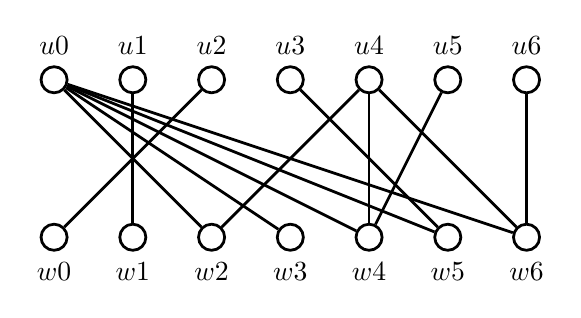
\begin{tikzpicture}[line width = 1pt,
                        solid/.style = {circle, draw, fill = black, minimum size = 0.1cm},
                        empty/.style = {circle, draw, fill = white, minimum size = 0.1cm}]
      \node [empty, label={above:$u0$}] (u0) at (0, 2){};
      \node [empty, label={above:$u1$}] (u1) at (1, 2){};
      \node [empty, label={above:$u2$}] (u2) at (2, 2){};
      \node [empty, label={above:$u3$}] (u3) at (3, 2){};
      \node [empty, label={above:$u4$}] (u4) at (4, 2){};
      \node [empty, label={above:$u5$}] (u5) at (5, 2){};
      \node [empty, label={above:$u6$}] (u6) at (6, 2){};
      \node [empty, label={below:$w0$}] (w0) at (0, 0){};
      \node [empty, label={below:$w1$}] (w1) at (1, 0){};
      \node [empty, label={below:$w2$}] (w2) at (2, 0){};
      \node [empty, label={below:$w3$}] (w3) at (3, 0){};
      \node [empty, label={below:$w4$}] (w4) at (4, 0){};
      \node [empty, label={below:$w5$}] (w5) at (5, 0){};
      \node [empty, label={below:$w6$}] (w6) at (6, 0){};
      \draw (u0) -- (w2); \draw (u0) -- (w3); \draw (u0) -- (w4); \draw (u0) -- (w5); \draw (u0) -- (w6);
      \draw (u1) -- (w1);
      \draw (u2) -- (w0);
      \draw (u3) -- (w5);
      \draw (u4) -- (w2); \draw (u4) -- (w4); \draw (u4) -- (w6);
      \draw (u5) -- (w4);
      \draw (u6) -- (w6);
    \end{tikzpicture}
    \end{center} \par
    \normalsize
    \item Yes. A perfect matching is
    \small
    \begin{center}
    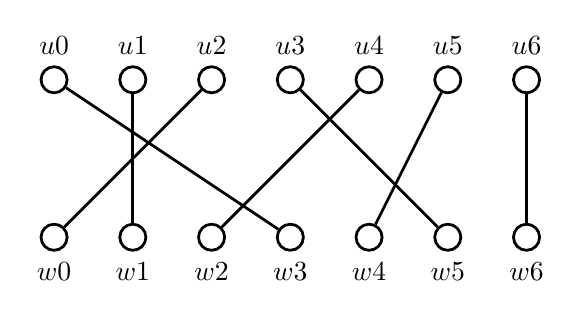
\begin{tikzpicture}[line width = 1pt,
                        solid/.style = {circle, draw, fill = black, minimum size = 0.1cm},
                        empty/.style = {circle, draw, fill = white, minimum size = 0.1cm}]
      \node [empty, label={above:$u0$}] (u0) at (0, 2){};
      \node [empty, label={above:$u1$}] (u1) at (1, 2){};
      \node [empty, label={above:$u2$}] (u2) at (2, 2){};
      \node [empty, label={above:$u3$}] (u3) at (3, 2){};
      \node [empty, label={above:$u4$}] (u4) at (4, 2){};
      \node [empty, label={above:$u5$}] (u5) at (5, 2){};
      \node [empty, label={above:$u6$}] (u6) at (6, 2){};
      \node [empty, label={below:$w0$}] (w0) at (0, 0){};
      \node [empty, label={below:$w1$}] (w1) at (1, 0){};
      \node [empty, label={below:$w2$}] (w2) at (2, 0){};
      \node [empty, label={below:$w3$}] (w3) at (3, 0){};
      \node [empty, label={below:$w4$}] (w4) at (4, 0){};
      \node [empty, label={below:$w5$}] (w5) at (5, 0){};
      \node [empty, label={below:$w6$}] (w6) at (6, 0){};
      \draw (u0) -- (w3);
      \draw (u1) -- (w1);
      \draw (u2) -- (w0);
      \draw (u3) -- (w5);
      \draw (u4) -- (w2);
      \draw (u5) -- (w4);
      \draw (u6) -- (w6);
    \end{tikzpicture}
    \end{center} \par
    \normalsize
    This means that there exists a permutation $\pi$ of $\{0, 1, 2, 3, 4, 5, 6\}$, such that $w_{\pi(i)}$ is a correct response to $u_i$, for $0 \leq i \leq 6$.
  \end{enumerate}

  \section{[GC] Problem 8.3}
  For graph $G_1$, $U$ can be matched to $W$. One possible matching is $\{(a, x), (b, w), (c, v), (d, z), (e, y)\}$. \par
  For graph $G_2$, $U$ can't be matched to $W$. Consider vertex set $\{b, d, e\}$, the cardinality of its neighborhood is only 2, which violates Hall's condition.

  \section{[GC] Problem 8.4}
  For all subset $U'$ of $U$, since every two vertices in $U'$ have distinct degrees, the maximum degree of all vertices of $U'$ is at least $|U'|$, and thus the cardinality of the neighborhood of $U'$ is at least $|U'|$. Therefore, the graph $G$ satisfies Hall's condition, which means $G$ contains a perfect matching.

  \section{[GC] Problem 9.6}
  \begin{enumerate}
    \item True. It is obvious that if a graph does not contain a subdivision of $K_5$ or $K_{3,3}$, neither does its subgraph. Therefore, by Kuratowski's Theorem, every subgraph of a planar graph is planar.
    \item False. For any nonplanar graph, if we take one of its vertices as a trivial subgraph, then it is obviously a planar subgraph.
    \item False. Consider $K_5$, removing any of its edges or vertices will make the resulting graph not contain a subdivision of $K_5$ or $K_{3,3}$, so $K_5$ is a counterexample to this statement.
    \item False. If we insert an vertex to any edge of $K_5$, the resulting graph does not contain $K_5$ or $K_{3,3}$ as a subgraph, however, it is still nonplanar.
    \item False. Consider the union of $K_5$ and $C_3$, with order $n = 8$ and size $m = 13$, which satisfies $m \leq 3n-6$. However, one of its components is nonplanar, and thus the graph is nonplanar.
    \item False. Consider the union of $K_{3,3}$ and $C_3$, it has a triangle and contains no subdivision of $K_5$ as a subgraph, however, it is  nonplanar.
  \end{enumerate}

  \section{[GC] Problem 9.13}
  \begin{enumerate}
    \item Since $G$ contains no triangle, the boundary of every region has at least 4 edges. Because every edge belongs to at most two of the boundaries, we have $2m \geq 4r$, i.e. $2r \leq m$. By Euler's Identity, we have $r=2+m-n$. Hence, $4+2m-2n \leq m$, i.e. $m \leq 2n-4$.
    \item For $K_{3,3}$, $n = 6$, $m = 9$, $m > 2n - 4$. Note that $K_{3,3}$ contains no triangle, so $K_{3,3}$ is nonplanar.
    \item This is true. First, $G$ contains no triangle because it is bipartite. Suppose that every vertex has degree 4 or more, then $2m \geq 4n$, i.e. $m \geq 2n$, which violates the inequality we proved in (a). Therefore, $G$ has a vertex of degree 3 or less.
  \end{enumerate}

  \section{[GC] Problem 9.14}
  \begin{enumerate}
    \item Since the length of a smallest cycle in $G$ is 5, the boundary of every region has at least 5 edges. Because every edge belongs to at most two of the boundaries, we have $2m \geq 5r$. By Euler's Identity, we have $r=2+m-n$. Hence $2+m-n\leq\frac{2}{5}m$, i.e. $m \leq \frac{5}{3}(n-2)$.
    \item Petersen graph has 15 edges and 10 vertices, so $m > \frac{5}{3}(n-2)$. Since the length of a smallest cycle in Petersen graph is 5, it is nonplanar.
    \item Removing any vertex of the Petersen graph yields a subdivision of $K_{3,3}$, so the Peterson graph is nonplanar.
    \begin{figure}[h]
        \centering
        \includegraphics{petersen_nonplanar.png}\\
    \end{figure}
    \item Suppose, to the contrary that every vertex of $G$ has a degree of 3 or more, then $2m \geq 3n$. Therefore, $\frac{3}{2}n \leq m \leq \frac{5}{3}(n-2)$. After some algebra we get $n \geq 20$, which leads to contradiction.
  \end{enumerate}

  \section{[GC] Problem 9.15}
  Suppose that every vertex of $G$ has degree 5 or more, then we have $2m \geq 5n$. Since $m \leq 3n - 6$, we have $n \geq 12$, which contradicts $n \leq 11$.

  \section{[GC] Problem 10.1}
  $\chi(G_1) = 3$; $\chi(G_2) = 4$; $\chi(G_3) = 4$; $\chi(G_4) = 3$; $\chi(G_5) = 4$.

  \section{[GC] Problem 10.4}
  \begin{enumerate}
    \item False. $K_4$ is a planar graph that contains a triangle, however, its chromatic number is 4.
    \item False. Consider $C_4$, it has a 4-coloring, however, it also has a 2-coloring, which means $\chi(C_4) = 2$.
    \item False. Consider $K_5$, it has no 3-coloring, but $\chi(K_5) = 5$.
    \item False. Consider $K_{3,3}$, since it is bipartite, its chromatic number is 2, but it is not planar.
  \end{enumerate}

  \section{[GC] Problem 10.10}
  Consider a graph whose vertex set are these subjects, and two vertex $i$, $j$ are joined by edge if and only if there exists some student who takes both the two subjects. The chromatic number is the minimum number of time periods needed for arranging all these subjects. \par
  In this case, the chromatic number of the graph is 4, and a possible 4-coloring is:
    \small
    \begin{center}
    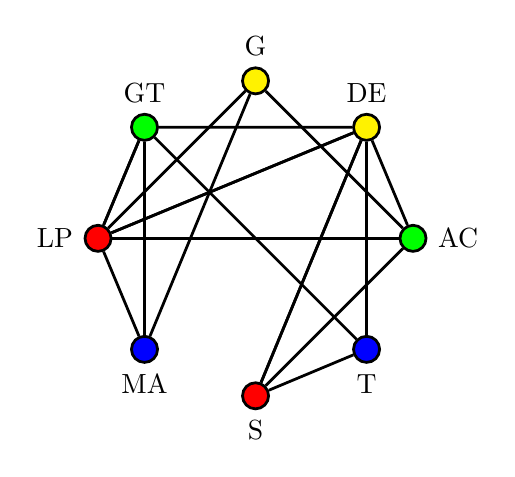
\begin{tikzpicture}[line width = 1pt,
                        empty/.style = {circle, draw, minimum size = 0.1cm}]
      \node [empty, label={right:AC}, fill=green] (AC) at (2, 0){};
      \node [empty, label={above:DE}, fill=yellow] (DE) at (1.41, 1.41){};
      \node [empty, label={above:G}, fill=yellow] (G) at (0, 2){};
      \node [empty, label={above:GT}, fill=green] (GT) at (-1.41, 1.41){};
      \node [empty, label={left:LP}, fill=red] (LP) at (-2, 0){};
      \node [empty, label={below:MA}, fill=blue] (MA) at (-1.41, -1.41){};
      \node [empty, label={below:S}, fill=red] (S) at (0, -2){};
      \node [empty, label={below:T}, fill=blue] (T) at (1.41, -1.41){};
      \draw (AC) -- (DE) -- (LP); \draw (AC) -- (LP);
      \draw (AC) -- (G) -- (LP);
      \draw (G) -- (MA) -- (LP);
      \draw (LP) -- (GT) -- (MA);
      \draw (DE) --(GT) -- (LP); \draw (DE) -- (LP);
      \draw (DE) -- (T) -- (GT);
      \draw (DE) -- (S) -- (T);
      \draw (AC) -- (S) -- (DE);
    \end{tikzpicture}
    \end{center} \par
    \normalsize
    so the earliest time that they can finish all exams is 4:45.

  \section{[GC] Problem 10.11}
  Consider a graph whose vertex set are these chemicals, and two vertex $i$, $j$ are joined by edge if and only if they react with each other. The chromatic number of this graph is the minimum number of containers needed for shipping. \par
  In this case, the chromatic number of the graph is 4, and a possible 4-coloring is:
    \small
    \begin{center}
    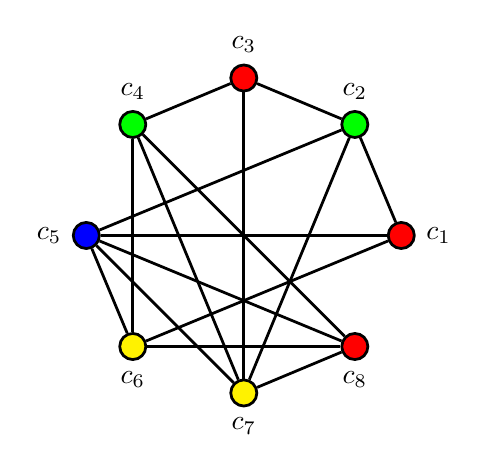
\begin{tikzpicture}[line width = 1pt,
                        empty/.style = {circle, draw, minimum size = 0.1cm}]
      \node [empty, label={right:$c_1$}, fill=red] (c1) at (2, 0){};
      \node [empty, label={above:$c_2$}, fill=green] (c2) at (1.41, 1.41){};
      \node [empty, label={above:$c_3$}, fill=red] (c3) at (0, 2){};
      \node [empty, label={above:$c_4$}, fill=green] (c4) at (-1.41, 1.41){};
      \node [empty, label={left:$c_5$}, fill=blue] (c5) at (-2, 0){};
      \node [empty, label={below:$c_6$}, fill=yellow] (c6) at (-1.41, -1.41){};
      \node [empty, label={below:$c_7$}, fill=yellow] (c7) at (0, -2){};
      \node [empty, label={below:$c_8$}, fill=red] (c8) at (1.41, -1.41){};
      \draw (c1) -- (c2); \draw (c1) -- (c5); \draw (c1) -- (c6);
      \draw (c2) -- (c3); \draw (c2) -- (c5); \draw (c2) -- (c7);
      \draw (c3) -- (c4); \draw (c3) -- (c7);
      \draw (c4) -- (c6); \draw (c4) -- (c7); \draw (c4) -- (c8);
      \draw (c5) -- (c6); \draw (c5) -- (c7); \draw (c5) -- (c8);
      \draw (c6) -- (c8);
      \draw (c7) -- (c8);
    \end{tikzpicture}
    \end{center} \par
    \normalsize
    so at least 4 containers are needed, and thus the minimum cost is \$380.
\end{document}
